\section{Normalized Path Difference Area (NPDA)}

Normalized path difference area (NPDA)\cite{mao2017segment,su2020survey} 
is a way to evaluate the shape similarity between the real and desired path. 
It is the difference area $A$ enclosed by two paths and 
divided by the length $L$ of desired path, $\text{NPDA} = A/L$.
This metric represents a similar idea to ALE that describes deviations from the 
given trajectory. Therefore, only ALE is reported in the paper.

\begin{figure}[H]
  \begin{minipage}{\textwidth}
    \centering
    \begin{tikzpicture}[inner sep=0pt,outer sep=0pt]
	  \node[anchor=south west] (pop) at (0in, 0in)
      {{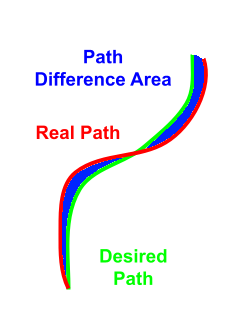
\includegraphics[height=1.5in,clip=true,trim=0.25in 0.1in
      0.25in 0.25in]{figs/NPDA_final.png}}};
    \end{tikzpicture}
    \vspace*{-7pt}
    \caption{The method to compute path difference area \label{fig:pda}}
  \end{minipage}  
  \vspace*{-1.5em}
\end{figure}

\subsection{Short Distance Simulation Outcomes}
\vspace*{-0.5em}
\begin{figure*}[h]
\begin{minipage}[t]{\textwidth}
\centering
%\vspace*{-1.45in}
\captionof{table}{ Short distance simulation NPDA outcomes.\label{tab:shortNPDA}}
\vspace*{-0.5em}
\begin{tikzpicture}[inner sep=0pt,outer sep=0pt,scale=1, every node/.style={scale=0.8}]
    % sim NPDA
	\node[anchor=north west] (sim_npda) at (0, 0pt)
    {
    \setlength{\tabcolsep}{4pt}
    \begin{tabular}{|c||c|cc|}
    \hline 
    \textbf{Seq.} & PO & SLAM & TS \\ 
    \hline 
%       &       &       & SLAM  & $\neg$SLAM \\
    SS  & 0.61  & 0.71  & 0.72  \\ 
    SWT & 0.63  & 1.12  & 0.88  \\ 
    SST & 0.51  & 1.47  & 0.59  \\ 
    STS & 0.73  & 1.33  & 0.75  \\ 
    STT & 0.66  & 0.93  & 0.80  \\ 
    \hline 
    \textbf{Avg.} & 0.63 & 1.11 & \textbf{0.75} \\ 
    %\textbf{Std. ATE} & 0.0000 & 0.0000 & 0.0000 \\
%    & \textcolor{white}{$v,\omega$} & & & \\
    \hline 
    \end{tabular}
    };
    
    \node[anchor=south, text width=5cm, text centered] (sim_npda_cap) 
    at ($(sim_npda.north) + (0pt, 2pt)$)
    {\normalsize \textbf{(a)} Sim NPDA (cm)};
      
    % p-values
    \node[anchor=west] (sim_npda_p) at ($(sim_npda.east) + (5pt, 0)$)
    {
    \setlength{\tabcolsep}{5pt}
    \begin{tabular}{|l||c|}
    \hline 
    \textbf{PO} vs \textbf{SLAM} & \textless 1e-5 \\ 
    \hline 
    \textbf{PO} vs \textbf{TS} & 2.2e-2 \\ 
    \hline
    \textbf{SLAM} vs \textbf{TS} & 8.4e-4 \\ 
    \hline 
    \end{tabular}
    };
    
	\node[anchor=south, text width=5cm, text centered] (sim_npda_p_cap) 
    at ($(sim_npda_p.north) + (0pt, 2pt)$)
    {\normalsize \textbf{(b)} p-values of \\ pairwise comparisons};        

\end{tikzpicture}
\end{minipage}
\vspace*{-1.5em}
\end{figure*}

\subsection{Long Distance Simulation Outcomes}
\vspace*{-0.5em}
\begin{figure*}[h]
\begin{minipage}[t]{\textwidth}
\centering
%\vspace*{-1.45in}
\captionof{table}{ Long distance simulation NPDA outcomes.\label{tab:longNPDA}}
\vspace*{-0.5em}
\begin{tikzpicture}[inner sep=0pt,outer sep=0pt,scale=1, every node/.style={scale=0.8}]
    % sim NPDA
	\node[anchor=north west] (sim_npda) at (0, 0pt)
    {
    \setlength{\tabcolsep}{4pt}
    \begin{tabular}{|c||c|cc|c|}
    \hline 
    \textbf{Seq.} & PO & SLAM & TS & TS+PO \\ 
    \hline 
%      & \textcolor{white}{$v,\omega$} & & \\
    LRU & 0.50  & 3.28  & 4.23  & 1.29 \\ 
    LLU & 0.84  & 9.35  & 6.03  & 1.42 \\ 
    LST & 1.10  & 7.50  & 8.94  & 2.54 \\ 
    LZZ & 0.93  & 10.31  & 4.54  & 7.60 \\ 
    \hline 
    \textbf{Avg.} & 0.84 & 7.61 & \textbf{5.94} & 3.21 \\
    \hline 
    \end{tabular}
    };
    
    \node[anchor=south, text width=5cm, text centered] (sim_npda_cap) 
    at ($(sim_npda.north) + (0pt, 2pt)$)
    {\normalsize \textbf{(a)} Sim NPDA (cm)};
      
    % p-values
    \node[anchor=west] (sim_npda_p) at ($(sim_npda.east) + (5pt, 0)$)
    {
    \setlength{\tabcolsep}{5pt}
    \begin{tabular}{|l||c|}
    \hline 
    \textbf{PO} vs \textbf{SLAM} & \textless 1e-5 \\ 
    \hline 
    \textbf{PO} vs \textbf{TS} & \textless 1e-5 \\ 
    \hline
    \textbf{PO} vs \textbf{TS+PO} & 1.1e-2 \\ 
    \hline 
    \textbf{SLAM} vs \textbf{TS} & 1e-1 \\ 
    \hline 
    \textbf{SLAM} vs \textbf{TS+PO} & 2.4e-3 \\ 
    \hline 
    \textbf{TS} vs \textbf{TS+PO} & 1.1e-2 \\ 
    \hline 
    \end{tabular}
    };
    
	\node[anchor=south, text width=5cm, text centered] (sim_npda_p_cap) 
    at ($(sim_npda_p.north) + (0pt, 2pt)$)
    {\normalsize \textbf{(b)} p-values of \\ pairwise comparisons};       

\end{tikzpicture}
\end{minipage}
  \vspace*{-1.5em}
\end{figure*}
